\pagina{Cierre de las evaluaciones exploratorias}
\label{sec:exploration}
\subsection{Selección dirigida y cierre de la entrega}
Se cerraron dos exploraciones complementarias a la evaluación distribuida. La primera utilizó las variantes guiadas en doce grafos reportados como resueltos por otro equipo y sin certificado en nuestro consolidado. Registró \PriorAttempts{} intentos, dos éxitos certificados y \PriorErrors{} interrupciones; encontró ciclos en graph4 y graph35. Se conserva como un protocolo separado de la evaluación distribuida.

La exploración v4 seleccionó 65 grafos todavía pendientes: 41 con mejor costo previo uno, 15 con costo dos y siete con costo tres, además de graph99 y graph85, con costos cuatro y cinco, que el otro equipo reportó resueltos. Se eliminaron duplicados y se excluyeron graph4 y graph35 por sus certificados ya disponibles. El costo previo procede de la evaluación distribuida, no de una distancia garantizada a una solución.

El protocolo fijó seis familias, diez semillas 2001--2010, hasta 30 segundos por intento y cuatro procesos independientes, con un hilo nativo por proceso y afinidad a las CPU lógicas 0, 2, 4 y 6 de la laptop de Arturo. No hubo límite de evaluaciones ni iteraciones; el límite externo fue de 90 segundos para incluir arranque y carga. Se admitió solo un intento simultáneo del mismo grafo. El orden priorizó los diez éxitos externos pendientes y después el costo previo.

La evaluación quedó cerrada en \RepairAttempts{} de las 3\,900 combinaciones previstas (\RepairCoverage\%). Se conservaron \RepairSuccesses{} éxitos, \RepairExhausted{} agotamientos y \RepairErrors{} interrupciones. Alcanzó \RepairStarted{} grafos: \RepairComplete{} completos y \RepairPartial{} parciales; otros \RepairUnstarted{} no se iniciaron. Las \RepairOmitted{} combinaciones no ejecutadas quedan fuera de la entrega y no se retomarán. Las incidencias del cierre permanecen en el denominador.

La sesión registrada duró \RepairSessionHours{} horas de reloj. Esta duración incluye coordinación y cuatro procesos concurrentes; no es una duración serial ni acredita aceleración frente a las etapas anteriores. Se volvieron a auditar los \RepairAttempts{} registros v4 y los \PriorAttempts{} de la exploración previa, comprobando artefactos, identidades, costo y ciclos sin ejecutar nuevamente los algoritmos.

\subsection{Éxitos y cobertura de los algoritmos}
La reparación v4 certificó cinco grafos adicionales: graph1, graph39, graph43, graph47 y graph52. El cuadro~\ref{tab:repairfamilies} conserva todos los intentos, mientras que su tasa balanceada y mediana temporal utilizan únicamente los \RepairComplete{} grafos completos: \RepairBalancedDenominator{} intentos por familia. Los cuatro parciales no alteran ese denominador.

\begin{table}[H]\centering\small
\caption{Cierre v4 por familia. Intentos, éxitos e incidencias corresponden al total; HC cuenta grafos distintos. Tasa balanceada y mediana de proceso usan los 48 grafos completos.}\label{tab:repairfamilies}
\begin{tabularx}{\linewidth}{Yrrrrrr}
\toprule
Familia & Intentos & Éxitos & Incid. & HC & Tasa bal. (\%) & Mediana (s) \\ \midrule
GA & 498 & 4 & 1 & 3 & 0.83 & 30.86 \\
SA & 497 & 0 & 1 & 0 & 0.00 & 30.86 \\
AS & 496 & 2 & 0 & 1 & 0.42 & 30.86 \\
ABC & 496 & 5 & 1 & 4 & 1.04 & 30.86 \\
DE & 495 & 0 & 1 & 0 & 0.00 & 30.86 \\
PSO & 494 & 0 & 0 & 0 & 0.00 & 30.86 \\
\bottomrule\end{tabularx}

\end{table}

ABC produjo cinco éxitos en cuatro grafos, GA cuatro éxitos en tres grafos y AS dos éxitos en un grafo. Sus coberturas se solapan: no se suman para obtener cinco grafos distintos. SA, DE y PSO no certificaron ciclos en esta exploración. Esos resultados no invalidan sus éxitos bajo el protocolo distribuido de 60 segundos y otra configuración.

\begin{figure}[H]\centering
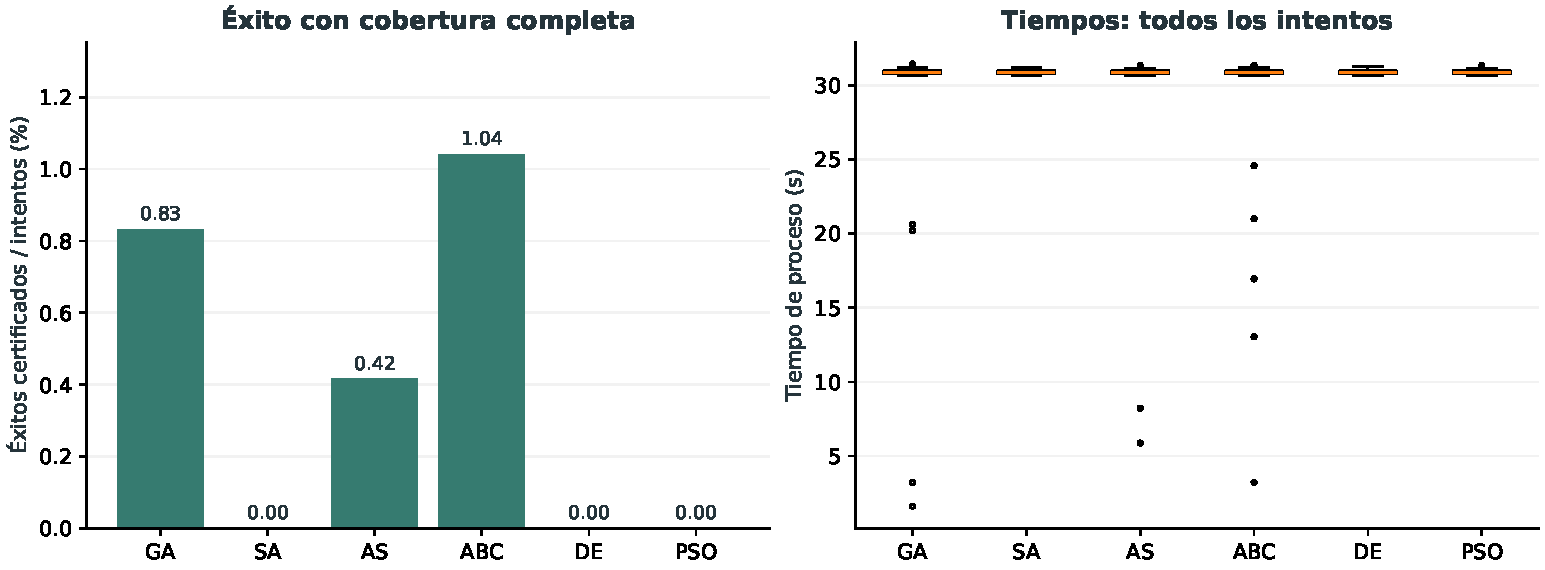
\includegraphics[width=\linewidth]{figures/exploratory-performance.pdf}
\caption{Exploración v4 en grafos completos: tasa de éxito y cajas de tiempo de proceso, con 480 observaciones por familia. Los tiempos incluyen intentos agotados; la mediana cercana al plazo no es un tiempo medio hasta resolver. Cajas: percentiles 25--75; bigotes: valores dentro de 1.5 rangos intercuartílicos; puntos exteriores conservados.}\label{fig:repairperformance}
\end{figure}

\begin{figure}[H]\centering
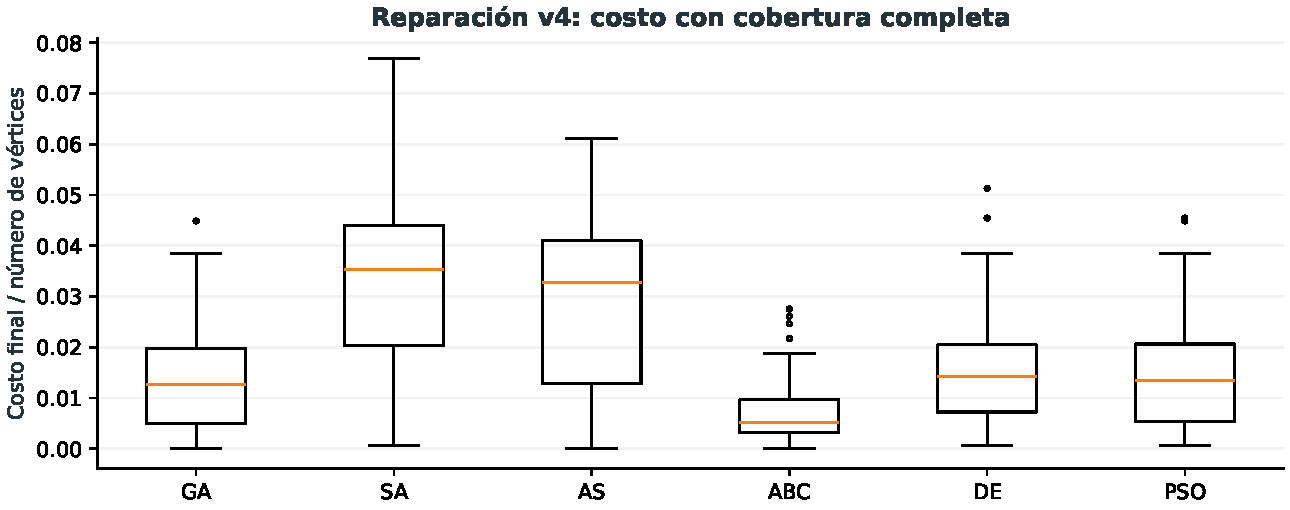
\includegraphics[width=.94\linewidth]{figures/exploratory-cost-boxplots.pdf}
\caption{Costo final normalizado por vértices en los mismos 48 grafos completos, con 480 candidatos por familia. Un costo positivo, aunque pequeño, no constituye ciclo. La convención de cajas es la de la figura~\ref{fig:repairperformance}.}\label{fig:repaircost}
\end{figure}

Los 41 grafos seleccionados por costo previo uno completaron sus 60 combinaciones. También se completaron los diez grafos pendientes reportados como resueltos por el otro equipo: cinco recibieron certificado propio; graph8, graph67, graph78, graph85 y graph99 agotaron sus combinaciones sin éxito. Los CSV externos aportan éxito declarado y dimensiones, pero no rutas para certificar sus soluciones ni condiciones equivalentes para comparar tasas.

Los parciales del cierre fueron graph60 (26 intentos), graph61 (25), graph66 (23) y graph71 (22). Quedaron sin iniciar graph77, graph83, graph86, graph88, graph89, graph115, graph154, graph25, graph73, graph76, graph117, graph123 y graph126. El anexo conserva costo previo/final y cobertura para los 65 seleccionados; no se presentan los no ejecutados como fallos.

\subsection{Balance de la entrega y límites de interpretación}
\begin{table}[H]\centering\small
\caption{Resultados por protocolo. Las filas conservan sus propios presupuestos y denominadores; no se calcula una tasa de éxito conjunta.}\label{tab:stagesclosed}
\begin{tabularx}{\linewidth}{Yrrr}
\toprule
Etapa & Intentos & Éxitos & Grafos HC \\ \midrule
M6: evaluación y escala & 900 & 0 & 0 \\
Evaluación distribuida & 8\,806 & 345 & 15 \\
Exploración guiada & 118 & 2 & 2 \\
Exploración con reparación v4 & 2\,976 & 11 & 5 \\
\bottomrule\end{tabularx}

\end{table}

\begin{table}[H]\centering\small
\caption{Siete grafos adicionales certificados en las exploraciones, ausentes del conjunto de 15 resueltos de la evaluación distribuida. Los conteos son intentos exitosos.}\label{tab:exploratorysolved}
\begin{tabularx}{\linewidth}{lYY}
\toprule
Grafo & Exploración & Éxitos por familia \\ \midrule
4 & Guiada & ABC: 1 \\
35 & Guiada & ABC: 1 \\
1 & Reparación v4 & ABC: 1, AS: 2 \\
39 & Reparación v4 & GA: 1 \\
43 & Reparación v4 & ABC: 2 \\
47 & Reparación v4 & ABC: 1, GA: 1 \\
52 & Reparación v4 & ABC: 1, GA: 2 \\
\bottomrule\end{tabularx}

\end{table}

La unión de los 15 grafos de la evaluación distribuida, los dos de la exploración guiada y los cinco de v4 contiene \UnionCertifiedGraphs{} grafos distintos certificados. Se superó así la referencia aproximada de 20 al considerar el conjunto de entregas, aunque la evaluación distribuida por sí sola conservó 15. La meta original de 60 no se alcanzó. La unión expresa cobertura acumulada, no una tasa comparable entre protocolos.

La selección se basó en resultados previos y éxitos externos; por tanto, presenta sesgo de selección y reutilización. Cambiaron operadores, semillas, presupuesto y concurrencia respecto a la evaluación distribuida. Los cinco ciclos adicionales demuestran soluciones válidas bajo v4, pero no aíslan el efecto causal de la reparación ni prueban superioridad estadística general. La ausencia de ciclos en otros intentos tampoco demuestra no hamiltonicidad.
